\chapter{Implementation}
\section{Design}
	Now that we had shown that a classifier could be built with relatively small sets of training data that still performed well, we had to design the interface to expose this functionality. This largely involved assessing tradeoffs between choices.
	
	\subsection{`Sketchy' or Formal}	
	\begin{figure}[h]
		\centering
		\begin{subfigure}[b]{0.4\textwidth}
			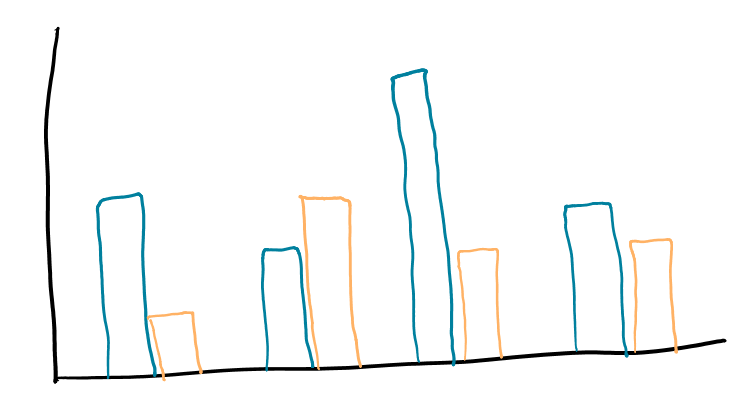
\includegraphics[width=\textwidth]{sketchy}
			\caption{Sketchy look}
			\label{fig:sketchy}
		\end{subfigure}
		\begin{subfigure}[b]{0.4\textwidth}
			\includegraphics[width=\textwidth]{formal}
			\caption{Formal look}
			\label{fig:formal}
		\end{subfigure}
	\end{figure}
	User content can be in shown in two styles: sketch or formal. This refers to the usability dimension described by \cite{bresciani_collaborative_2008} as 'Perceived Finishedness'. \cite{yeung_effect_2008} showed that a doodle-like appearance of low-fidelity prototypes encourages early-stage experimentation and discussion, whereas a formal appearance looks finished and professional.  Thus, we had to choose whether the system should generate the rest of the chart with a 'sketchy' look, or convert the input into a finished chart with a formal look. \cite{blackwell_formality_2008} note how the rapid replacement of pen and paper by computers has made more of our processes formal and precise, potentially discouraging us from exploration and iteration in creative processes that would benefit from them.
	
	Generating the 'sketchy' look can be non-trivial, \citep{plimmer_sketchnode:_2010, wang_sketchset:_2011} e.g.\ if the user draws one bar, how should the system generate more bars that look hand-drawn by the same author but not just like stretched versions of the first bar? Additionally, if the users want to present these charts to an audience, they must look polished, and so at some point an export option for a formal look needs to be offered. Thus, we decided to offer a hybrid that shows the user's input in sketch form, with the system's output in formal form. Extensions were implemented to keep these two forms as closely in synchronization as possible, thus making the mapping visually evident.
	
	\subsection{Sketches or gestures}
	A related design decision was whether to use sketches or gestures. Sketches share some visual semblance with the chart they're trying to indicate, whereas gestures are just movements chosen from a library of easy-to-distinguish movements, that behave like commands instructing the software to choose a certain chart type. SketchInsight \citep{walny_understanding_2012} uses the latter approach, requiring just an `L' shape to indicate a bar chart, or a `V' shape to indicate a line chart. 
	
%		\begin{tabular}[h]{p{0.5 \linewidth} | p {0.5 \linewidth}}
%			\bfseries{Pros} & \bfseries{Cons} \\
%			This would provide higher recognition accuracy, since the domain of shapes to distinguish between is limited, and can be designed to maximise differences between them. & One of the principles of direct manipulation is to avoid using a command language, but a gesture library is exactly that, requiring users to remember which gesture corresponds to which chart type or element. \\ \hline
%			& A gesture is transient, unlike a sketch. Users wouldn't be able to modify their input, they would have to redo their actions. 
%		\end{tabular}	
		
			\textbf{Pros}
			\begin{itemize}
			\item This would provide higher recognition accuracy, since the domain of shapes to distinguish between is limited, and can be designed to maximise differences between them. 
			\end{itemize}
			
			
			\textbf{Cons} 
			\begin{itemize}
			\item A gesture is transient, unlike a sketch. Users wouldn't be able to modify their input, they would have to redo their actions. 
			\item One of the principles of direct manipulation is to avoid using a command language, but a gesture library is exactly that, requiring users to remember which gesture corresponds to which chart type or element. 
			\end{itemize}
				
	
	This would provide higher recognition accuracy, since the domain of shapes to distinguish is much more limited, and can be designed to maximise differences between them. 
	
	% Can cite Chao
	\subsection{Modes or modeless}
	Since the application now has both sketch and formal content, the user must have an easy way to switch between the two views. One approach is to give the user an explicit UI widget to toggle between the two modes. This way, the user explicitly indicates what they want to see, and thus should have a better understanding of what state the system is in. This also allows the system a chance to change the controls available to the user.
	
	The other approach is to avoid modes, requiring lesser cognitive effort from the user since they don't need to keep track of what state the system is in. In this project, this could have been done by showing the sketch view when the user was about to edit the chart. The active digitizer hardware allows the system to detect when the user brings the stylus within range of the screen, just before they actually touch the screen, allowing the chart to be in sketch view by the time the stylus is down. When the stylus goes out of range, the system can switch to the formal chart view. This would solidify the metaphor that edits are done to the sketch, but the final product to be looked at is the formal view. 
	
	At first, the modeless version was chosen for its lower cognitive overhead. However, when the extension to allow edits not just to the sketch view, but also the formal view, was undertaken, we had to switch over to a mode-based system to allow the user to interact with the graph in both views with their stylus.
	
	\subsection{Stock or bespoke charting widget}	
	Since the system is generating a formal version of the chart, a charting component is required to render this visualisation. The .NET framework comes with built-in chart controls that offer basic functionality with relatively low implementation effort. They also allow easy export as dynamic chart objects into Microsoft Office files. However, customising their appearance beyond a certain point is extremely difficult, making it easier to just make one's own charting component from scratch and control all aspects of the rendering. This means having to re-implement a lot of core functionality though, such as scaling shapes correctly, choosing labels that are round figures when possible, and generating colours than work well together for different data series. This also means that the chart can only be exported as a raster image rather than as a chart object.
	
	To enable rapid prototyping, we chose to utilise the standard charting component at first. As our needs to customise the chart grew, we were able to make our own chart class that implemented the same interface as the standard component, and so could be slotted in to replace it.
	
	\subsection{Finite or infinite domain}
	Some tools, such as Microsoft Excel, let the user make one of a limited set of charts, such as bar or pie charts, quickly. Others, (which usually involve coding), such as D3.js, let the user make a vast variety of visualisations by creatively combining basic elements like lines, boxes and wedges. However, these require expert knowledge of the tools, and take longer to create basic visualisations. 
	
	\begin{table}[h]
	\begin{tabular}{p{0.15 \linewidth} p{0.425 \linewidth} p{0.425 \linewidth}}
	
									& 
	\bfseries Library of charts 	& 
	\bfseries Modular charts 		\\
	
	\textbf{Description} 																&
	Draw basic gestures or elements to indicate which chart type is desired 	& 
	Draw any one of 7 basic components and 
	bind data to attributes of theirs such as width, height, colour or radius
	\vspace{6 \lineskip} 	\\
	
	\textbf{Domain} 				&
	Finite domain 		& 
	Infinite domain 	\\
	
	\textbf{Speed} 				&
	Quick				& 
	Slower 				\\
	
	\textbf{Complexity}															&
	Simple interface, just drop data on an element to bind data			& 
	Complex interface to expose all attributes and manage data binding 	\\
	\end{tabular}
	\end{table}
	
	\cite{chao_poster:_2010} uses pen gestures to indicate 'proto-objects' that can be combined. While an infinite domain system that uses pen sketches would have been intriguing to explore, it would contradict the project's primary usability goal that the system should be faster than users' current systems. Additionally, the 80/20 rule indicated that while a few power users may want to generate custom visualisations, the majority would just want to make simple charts. Thus, the additional functionality didn't justify the additional complexity for the average user.
	
%	\subsection{To beautify or not to beautify}
%	The formal graphics generated by the system are easy to modify with existing tooling, whereas human ink strokes are less straightforward to modify while maintaining their natural look and feel.


	\section{Development}
	Interleaved with the design process above was the development process detailed in this section. The C\# code supports a stand-alone Sketch Chart component that can be used in any Windows Forms application that requires charting functionality, as well as a reference implementation of such an application, Sketchography, which lets users import their Microsoft Excel or Comma Separated Values data and generate charts. This satisfies all the core requirements described in \autoref{sec:Requirements}, as well as 3 of the 6 extensions outlined.
	
	\begin{figure}[h]
		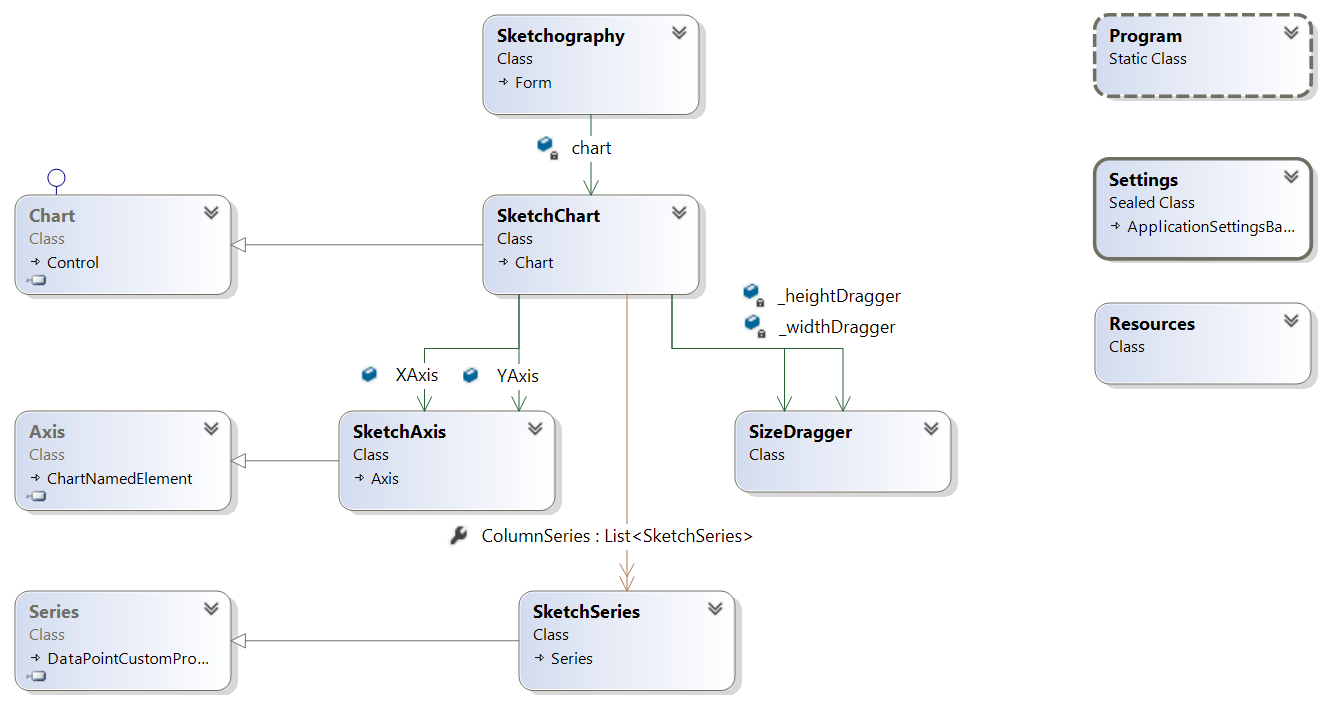
\includegraphics[width=1\linewidth]{ClassDiagram}
		\caption{Interactions between classes}
	\end{figure}		
	
	As seen above, the Sketchography form is the main application run when Program starts. Sketchography contains a SketchChart component, which contains the canvas for users to sketch on, as well as the formal chart generated. SketchChart in turn uses SketchAxis and SketchSeries objects. SketchChart, SketchAxis and SketchSeries inherit from their non-sketch counterparts Chart, Axis and Series (from System.Windows.Forms.DataVisualization.Charting, which is part of the .NET framework), in order to reuse the built-in functionality and members, and complement them with functions and members specific to sketching. SketchChart also references two instances of SizeDragger, which is a custom UI widget to support dragging ends of columns in a column chart to scale them. Settings and Resources are two additional classes used to store properties of the project.
	
	
	%TODO Should I include that the core of the project is around 620 lines of code? This doesn't include the classifier or the interface code
	No class is more than 400 lines of code, indicating that functionality has been split up at a reasonably fine grain to not concentrate too much responsibility in any one class. Visual Studio's calculated code metrics show that the project has a maintainability index of 74/100, which gets the highest rating - 'good' maintainability. Should I include the data in this paragraph?
	
	At a high level, the functionality of the program can be divided into 3 responsibilities - data handling, sketch processing and charting (in increasing order of complexity). It is written in an Object Oriented fashion, with separation between the views (Windows Forms) and controllers (C\# classes), to allow for easy testing.
	
	
	\subsection{Data import and management}
		Since the application is targeted at the average user, their data is most likely to be stored in spreadsheet format. Thus, it is important to allow them to import data from .xlsx and .csv files. 
		For the sake of simplicity, the code assumes that the data is well-formed. Specifically, it works on the following assumptions:
		\begin{enumerate}
		\item The data is arranged as records in the rows of the spreadsheet.
		\item The first row contains the names of the various fields.
		\item No data is missing (if there are $m$ columns and $n$ rows, there are $m \cdot n$ data values.
		\end{enumerate}
		
		Under these assumptions, importing tabular data is a common use case, so I studied a number of existing libraries and methods to do this in C\#. At first the LinqToExcel package from the NuGet package manager was used to easily import data from the file. However, this package had limited documentation, making it hard to achieve more complex tasks. Additionally, it added an external dependency, and carried a license that allow free reuse of the software as long as the original copyright message was included. The package was helpful for rapid prototyping at first, but after the code was more mature, we removed this dependency and implemented the file import ourselves using the OLE DB provider.
	
	%TODO Try to lay these screenshots out better, and decide whether first 2 are needed at all.
	\begin{figure}[h]
		\centering
		\begin{subfigure}[b]{0.3\textwidth}
			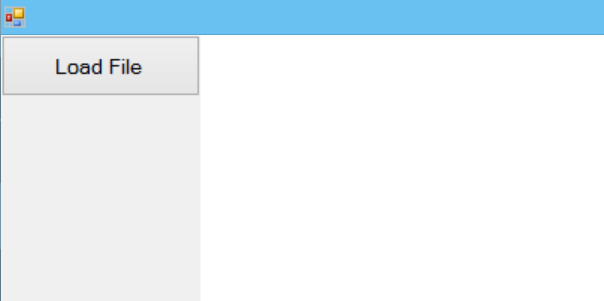
\includegraphics[width=\textwidth]{data1}
			\caption{Initial state}
			\label{fig:data1}
		\end{subfigure}
		\begin{subfigure}[b]{0.6\textwidth}
			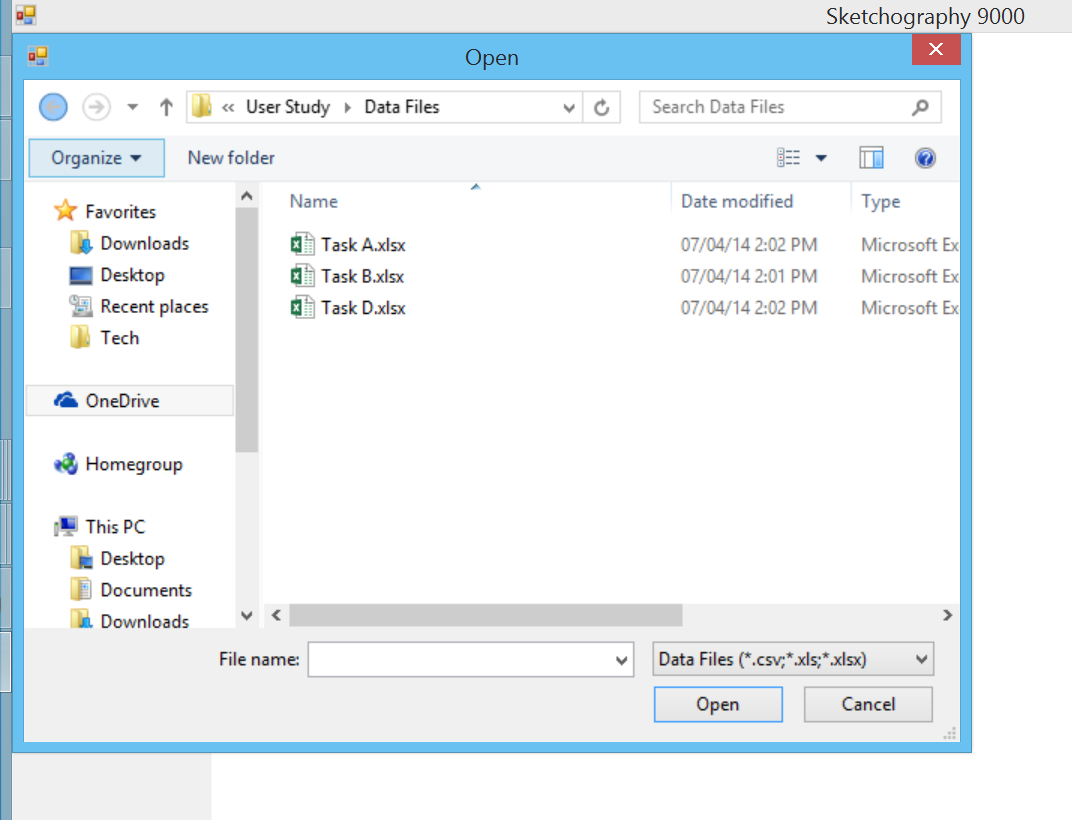
\includegraphics[width=\textwidth]{data2}
			\caption{When "Load File" is clicked}
			\label{fig:data2}
		\end{subfigure}
		\begin{subfigure}[b]{0.5\textwidth}
			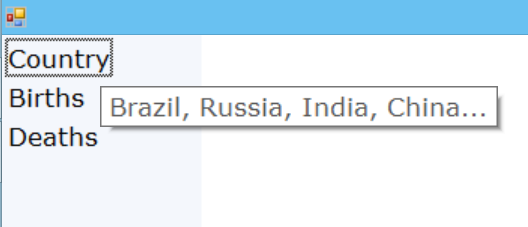
\includegraphics[width=\textwidth]{data3}
			\caption{Column headers are shown with data previews in tooltips}
			\label{fig:data3}
		\end{subfigure}
	\end{figure}		
		
		
	The interface shows a "Load File" button, which when clicked reveals a standard system filepicker dialog with a filter to show *.csv, *.xls and *.xlsx files.	Selecting a file causes the "Load File" button to disappear and be replaced by a list of column headers (the names of the various fields). This helps minimise interface clutter and only expose the most relevant information at all times. However, it comes at the cost of the user needing to hit 'Reset' if they choose the wrong file by mistake. To reassure the user that data has been imported correctly, and for them to check which column header corresponds to which data, hovering over any header reveals the first few entries for that field as a sample.
	
	
	\subsection{Sketch Processing Workflow}
	RATA.SSR provides a sample that calls the classifier API. For this project, that reference was followed, with a lot of extraneous code and unnecessary branches removed, until a basic prototype existed consisting of nothing but a blank canvas which receives user ink, passes it off to a classifier, and outputs the recognition result in a log-like text box. This was then integrated into the application described above, with its data import facility. 
	
	When the user draws a stroke on the SketchChart element within the Sketchography window, a number of steps occur:
	\begin{enumerate}
	\item The \texttt{SketchChart} is covered by an \texttt{InkOverlay} object, which receives the stroke. An \texttt{inkOverlay.Stroke} event is fired, which allows our event handler to run custom code.
	\item The \texttt{InkOverlay.Stroke} event handler calculates additional features of the stroke that are not included in the stroke's properties by default, and stores them in its extended properties.
	\item The stroke is then sent to the classifier, which is loaded from a file on program initialization.
	\item The \texttt{classifierClassify} function returns a string from a set of previously defined strings representing the various recognition results. This string is passed off to the \texttt{ConvertToFormal} method, which, as the name suggests, creates the corresponding formal chart elements. The \texttt{ConvertToFormal} method is also sent the stroke object itself, so that it can use its properties such as the location to place the formal object accordingly.
	 
	\end{enumerate}

	After the core of the project was finished, an extension was implemented that allows erasing of strokes. The stylus available has a button simulating an eraser at the back. When this eraser comes into range, a \texttt{CursorInRange} event is thrown, wherein we can check whether the stylus is inverted or not.
	
	\begin{lstlisting}[frame=single]
_inkOverlay.EditingMode = e.Cursor.Inverted ? 
		InkOverlayEditingMode.Delete : 
		InkOverlayEditingMode.Ink;
	\end{lstlisting}
	
	Then, when a stroke is received (the same event is thrown whether the stroke is ink or the eraser), if the editing mode is Ink, the steps above are run. If it is Delete, the corresponding chart element is detected and reset. On the next re-paint of the interface, this element will be removed from the canvas. To minimize lag between the action and the feedback, this repainting is forced immediately with an \texttt{Invalidate()} call.
	
	 Below is a description of how \texttt{ConvertToFormal} responds to user actions it receives, via the stroke classifier. 
	
	\begin{tabular}{p{0.2 \linewidth} p{0.8 \linewidth}}
	\bfseries User Action	& \bfseries Application Response \\
	Load File &
	Bind chart's data source to the in-memory data table created from the imported file. 
	\\
	
	\vspace*{10\lineskip}
	Draw an axis &
	\begin{enumerate}
	\item Calculate the bounding box (the smallest rectangle that entirely encloses the stroke) of the sketched axis, and use a heuristic comparing the height to the width to determine whether it is a vertical or horizontal axis. 
	\item The line running through the center of the bounding box is taken as the intended coordinates of the formal axis. This must be done since sketched axes are rarely perfectly straight lines, so using the actual endpoints of the line might result in a non-aligned axis. 
	\item The endpoint coordinates of the straightened line are used to set the vertical or horizontal position and size of the formal chart. They are also saved in an Axis object, which can then be drawn onto the formal chart.
	\item If it a horizontal axis, a drop target is below the axis. This is a rectangle of the same length as the axis, and a preconfigured height deemed big enough to make it hard for the user to miss, while minimising the screen space used up.
\end{enumerate}		
	\\
	
	\vspace*{10\lineskip}
	Draw a bar &
	\begin{enumerate}
	\item A bar is the indicator that the user wants a new data series added on a bar/column chart. Thus, a new data series is added to the chart's SeriesCollection in the form of a Series object. The name of this series is set as ``SeriesX'', where X is incremented for each new series. This will be useful for the drop target system described later.
	\item When the new series is added, the Chart object automatically assigns it a new series colour from the colour palette. The application changes the colour of the stroke the user drew to this series colour, to give feedback that it has been recognised as a series. 
	\item A drop target the same size and position as the bounding box of the bar is created, corresponding to that series.
	\end{enumerate}
	\\
	\end{tabular}

	\begin{figure}[h]
		\centering
		\begin{subfigure}[b]{0.4\textwidth}
			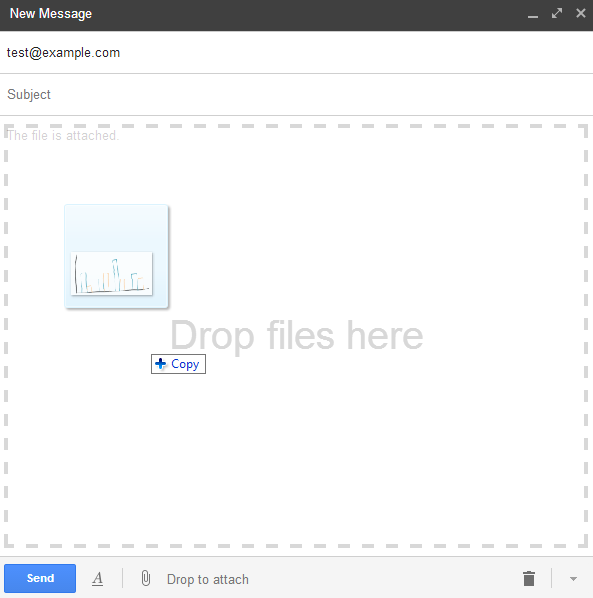
\includegraphics[width=\textwidth]{dropexample1}
			\caption{Gmail.com compose window, taken in May, 2014}
			\label{fig:dropexample1}
		\end{subfigure}
		\begin{subfigure}[b]{0.4\textwidth}
			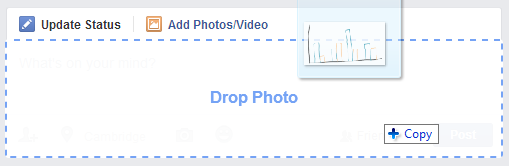
\includegraphics[width=\textwidth]{dropexample2}
			\caption{Facebook.com status update widget, taken in May, 2014}
			\label{fig:dropexample2}
		\end{subfigure}

	\end{figure}
	
	In response to strokes that create chart elements, drop targets are generated so that the user may then drag and drop data directly onto the chart element to bind it. This provides direct manipulation, since it doesn't force the user through a menu and dialogue system to configure which data corresponds to which axis. In order to do this, a dictionary is maintained in SketchChart, storing the mapping between Rectangles encoding the location of a drop target, and the string representing the chart element it corresponds to. For the x axis, this would be ``X Axis"; for the data series it would be the name of the series. 
	
	\begin{figure}[h]
	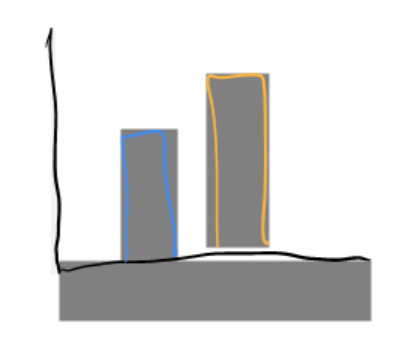
\includegraphics[scale=1]{droptargets}
	\caption{Drop Targets for 2 data series and the X axis, revealed when data is being dropped onto the chart}
	\end{figure}
	
	When the user begins dragging a column header from the list on the left, this calls a number of event handlers in Sketchography. These configure the drag and drop action so that the column name saved within the list item is the data sent to the drop location. They also flip a \texttt{ShowDropTargets} flag, so that the chart rendering system draws grey rectangles indicating where the drop areas lie. This UI pattern is based on one users may be familiar from a number of drag and drop interfaces they may have previously interacted with, thus making it easier for them to understand what's happening. We also tried adding `Drop here' text in the targets like in the examples below, but this proved to cluttered in the small drop targets being used. Additionally, hallway testing revealed that once users began dropping, they were already aware that they must drop it in targets, and the change in colour was conspicuous enough to draw their attention to them.
	
	When the data is dropped, this calls another event handler. In Sketchography, the event handler simply verifies that its a valid drag and drop, and then passes on the data to the \texttt{DropData} function on the SketchChart. For every rectangle in the dictionary of drop targets, \texttt{DropData} checks if the drop event occured within it. When it finds the drop target the user picked, it looks up the corresponding string, and calls \texttt{BindDataSeries} on it. \texttt{BindDataSeries} adds the binding appropriately. If the data was dropped on a data series rather than the X axis, it also renames that series and the corresponding drop target, so that the user can reassign that bar to some other data if they change their mind. From this point, the charting functionality takes over.
	
	
	
	
	

	
	\subsection{Charting}
	This part of the functionality, unexpectedly, proved the most challenging and time-consuming. In the first few iterations, a built-in .NET chart component was used, which allowed rapid prototyping. However, converting from the coordinate system used within the charting component to that used in the rest of the window was proving non-trivial and inaccurate. In addition, the component didn't allow very fine-grained positioning of its various elements, or much control over their sizing and other attributes. Hence, we had to implement our own chart control. To make the most of the functionality already implemented in the built-in control, we inherited from it. This also meant our custom control could easily replace the built-in one since it implemented the same interface but with a few extra features.
	
	The painting of the chart graphics is done in a largely procedural fashion unfortunately, as this is how it is done for Windows Forms controls. Most of the work is done in the \texttt{PostPaint} event handler, which is called after the built-in chart is done painting (even though the built-in chart control is not shown to the user at all, it still needs to be painted in a hidden background for some of its functionality to work correctly). This painting occurs whenever changes are made that might affect its output. Within the event handler, there are distinct sections that:
	\begin{itemize}
	\item Draw a background to cover up the built-in chart.
	\item Draw the formal axes and bars.
	\item Draw a height drag handle if needed.
	\item Draw a width drag handle if needed.
	\item Move the user's strokes to fit the bars.
	\item Draw the drop targets if needed.
	\item Change the colour of ink strokes to match their series colour if needed. 
	\item Update the legend.
	\end{itemize}
	
	Each of these steps involves a lot of complicated computation, maintaining of state, and conversion between coordinate systems. The particularly interesting parts are described below.
	
	\subsubsection{Positioning and scaling bars}
	To allow maximum flexibility, constants are introduced that control various parameters of the appearance of the bars, such as the ratio of the gap between them, and the fraction of the height of the chart they should cover by default. Then, formulae are used to account for the number of data series, the relative width scale of each series, the relative scale of the gap between data points, and the length of the X axis, to calculate the position each bar should be drawn at.
	
	The application also has to calculate the values to show for labels on the Y axis. This is something that the custom charting control doesn't handle as elegantly as the built-in control, since the values are not usually rounded, whole numbers. This is because the range of values in the data series is simply spread across a set number of labels to determine the individual label values.
	\subsubsection{Transforming strokes to match formal bars}
	\begin{figure}[h]
		\centering
		\begin{subfigure}[b]{0.35\textwidth}
			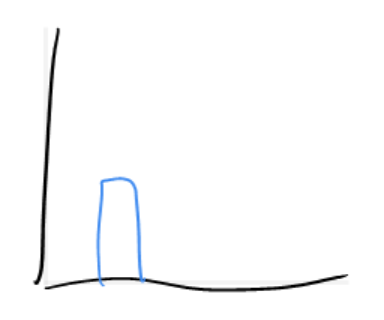
\includegraphics[width=\textwidth]{sketchtransform1}
		\end{subfigure}
		\begin{subfigure}[b]{0.4\textwidth}
			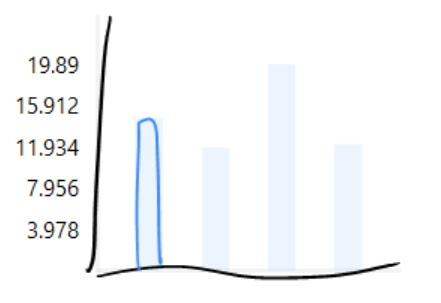
\includegraphics[width=\textwidth]{sketchtransform2}
		\end{subfigure}
		\caption{Before and after the transform}
	\end{figure}		
	
	This was implemented as an extension, to better express the connection between the sketches and the formal bars to the user. It is done by maintaining a mapping between the sketch and the first bar of the series. When the bar is drawn, its coordinates and dimensions are saved. These are then applied as a scale and translation transform to the associated sketch.
	
	
	\subsubsection{Height and width dragging}
	Another extension was to allow users to make changes to the formal chart, and have those changes feed back to the sketches. We decided to offer the ability to change the width and height of the bars. When in the formal view, if users hover over the first bar in a series, they see a drag handle each for the height and width, in the form of a grey rectangle. We decided on the size of these handles by experimenting with various sizes to see which one formed a target big enough to grasp with a stylus. Since these rectangles are simply graphics drawn onto a picture box rather than explicit controls, they do not offer native drag functionality. Instead, this has to be approximated by toggling a flag when mouse/stylus is down within the rectangle of the drag handle indicating that a drag has started. When the mouse/stylus is lifted, if the flag was on and the cursor position has changed, this is viewed as a drag, and the change in position is taken to be the size change desired. This scaling is then applied to the variables previously introduced for positioning and scaling bars, so the changes take effect in the next paint cycle, which seems fairly instantaneous to users, if not perfectly so.
	
	\begin{figure}
	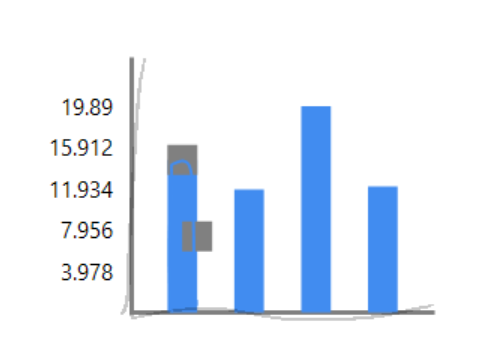
\includegraphics[scale=1]{draghandles}
	\caption{Drag handles}
	\end{figure}		
	
	To help users discover what these drag handles do, the cursor changes to a sideways drag cursor in the direction corresponding to whether it is a height or width handle, when it hovers over these handles.	
	
	At first, the naive implementation of the scaling broke when users tried particularly extreme drags, which they tended to play with even if it wasn't the scale they finally intended to use. The calculations had to be refined over time.
	
	\subsubsection{Maintaining the legend}
	To keep the user aware of the state of the system at all times, it is important to have a legend showing which data is connected to which element of the visualisation. While most charting tools have a separate legend, we decided, in the theme of direct manipulation, that the colour key should be right where the data is - in the list of column headers. 
	
	However, the list of column headers is in the Sketchography form, whereas the colours are stored within the SketchChart, which is referenced in the form. We followed a subscriber pattern here, by creating an event in SketchChart that notifies about changes to the legend. SketchChart also exposes a public Legend dictionary, mapping colours to headers. Sketchography subscribes to those notifications, and its event handler regenerates the legend by checking the list in SketchChart.	
	
	\begin{figure}
	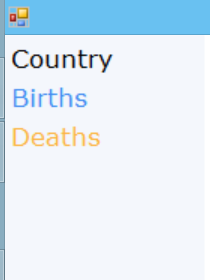
\includegraphics[scale=1]{legend}
	\caption{Legend}
	\end{figure}
	
	
	\subsubsection{Switching between the formal and informal views}
	We initially did this by offering a simple toggle button that read `Toggle View', and a text box that showed the current view the user was in `Sketch View' or `Chart View'. However, during hallway testing, users repeatedly clicked on the text box, or were just generally confused about which view they were in. This confirmed a previous worry that the disconnect between the action trigger and the reflection of its actions would be confusing, so we implemented radio buttons as shown below. These contain pictures of the two views, so users can spot the difference visually without needing to internalise what the two phrases represent. Another concept of showing visual layers with live previews was not tested because of time and technical constraints.
	
	%TODO Get screenshot of earlier iteration
	
	\begin{figure}[h]
	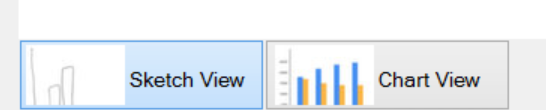
\includegraphics[scale=1]{toggle}
	\caption{Switching between formal and informal views}
	\end{figure}
	
	Behind the scenes, all the chart elements are drawn in both views, with the unselected view dimmed or ghosted out. Hence, when users are sketching, they can see faint feedback of the recognition in the background and thus notice early if there has been a misclassification. This is done by setting two alpha or transparency values - one which is high when the formal view is selected, and one which is high when the in informal mode. Each of the elements then uses one of these alpha values to draw themselves according to which mode they should be prominent in.